\documentclass[11pt, conference, compsocconf]{IEEEtran}
\usepackage{amsmath}  
\usepackage{braket}
\usepackage{tikz}
\usetikzlibrary{shapes.geometric, arrows}
\tikzstyle{startstop} = [rectangle, rounded corners, minimum width=3cm, minimum height=1cm,text centered, draw=black, fill=red!30]
\tikzstyle{io} = [trapezium, trapezium left angle=70, trapezium right angle=110, minimum width=3cm, minimum height=1cm, text centered, draw=black, fill=blue!30]
\tikzstyle{process} = [rectangle, minimum width=3cm, minimum height=1cm, text centered, text width=3cm, draw=black, fill=orange!30]
\tikzstyle{decision} = [diamond, minimum width=3cm, minimum height=1cm, text centered, draw=black, fill=green!30]
\tikzstyle{arrow} = [thick,->,>=stealth]



\begin{document}

\title{Variational Monte Carlo}
\author{\IEEEauthorblockN{Christopher Parker}
\IEEEauthorblockA{Computational Physics Department\\
University of Oslo\\
%Huntsville, Alabama\\
csparker.work@gmail.com}
}
\maketitle

\begin{abstract}
Final project on variational Monte Carlo for FYS 3150. Code available at github.com/csp256/FYS3150\_Final\_Project\end{abstract}

\IEEEpeerreviewmaketitle


\section{Introduction}
The aim of this project is to use Variational Monte Carlo (VMC) to place upper bounds on the ground state energy of closed shell systems of harmonic potential. The number of electrons N necessary to create a closed shell system is a combinatorics problem dependent upon the number of dimensions D to be considered. We restrict ourselves to the first two closed shells of two dimensions, N=2 and N=6, as unresolvable singularities prevent a solution in one dimension. The N=2 case trivializes considerations arising from spin that are addressed in the N=6 case. We numerically recover correct ground state energy values, and note an interesting, unexplained, but corraborated result regarding the virial ratio of kinetic to potential energy.

\section{Physical Principles}
Natural atomic units are assumed throughout this work: physical constants are set to 1.

\subsection{Variational Principle}
The Schrodinger equation, when formulated as an eigenvalue problem, is:
\begin{align}\hat{H}\ket{\psi} &= E\ket{\psi}\\
\bra{\psi}\hat{H}\ket{\psi} &= E\bra{\psi}\ket{\psi}\\
\bra{\psi}\hat{H}\ket{\psi} &= E
\end{align}
If we consider the ground state energy $E_{gs}$ and any arbitrary normalized function $\psi_{T}$ (the trial wavefunction), which is not necessarily an eigenfunction, then the variational principle states:
\begin{align}\bra{\psi_{T}}\hat{H}\ket{\psi_{T}} &= E_T \geq E_{gs}\end{align}
Where the proof follows from the eigenfunctions of $\hat{H}$ forming a complete set, where the trial wavefunction may be expressed as a linear combination of these eigenfunctions. Without the normalization condition a wavefunction $\psi_{T'}$ might have a lower energy, by having arbitrarily small coefficients on each of the eigenfunctions. Normalization restricts this so that the least energetic way to "distribute" the coefficients to each term is to assign 0 to every eigenfunction except the ground eigenfunction, which is assigned 1: any other choice of coefficients (any other wavefunction) is more energetic.

We may then, with great freedom, chose trial wavefunctions in a manner apropriate to our system.

\subsection{Eigenfunctions Of Harmonic Potential}
With harmonic potential: 

\begin{align}V\left(r\right)=\frac{1}{2}\omega r^2\end{align} 

The single particle Hamiltonian (obviously but notably without inter-electron repulsion) becomes: 

\begin{align}\hat{H_0} \left(r\right)=-\frac{1}{2}\nabla^2 + \frac{1}{2}\omega r^2\end{align}

Which has (for suitable, discrete values of $\omega$) eigenfunctions in two dimensions of:

\begin{align}\phi_{n_x,n_y}\left(r\right) = H_{n_x}\left(\sqrt{\omega}x\right) H_{n_y}\left(\sqrt{\omega}y\right) exp\left(-\frac{1}{2}\omega r^2\right)\end{align}

Where $H_n\left(x\right)$ are the Hermite polynomials. We then define $k \equiv \sqrt{\alpha \omega}$ and use $k$ in leiu of $\sqrt{\omega}$, where $\alpha$ is a variational parameter introduced to tweak the trial wavefunction. This is discussed further in a later section.

Without inter-electron repulsion the Hamiltonian (and eigenfunctions) for multi-electron systems is simply formed by adding multiple single particle Hamiltonians. With inter-electron repulsion (truncated to two body interaction) the form of the Hamiltonian becomes:

\begin{align}\hat{H} = -\sum\limits_i {\frac{1}{2}\nabla_i^2} + \sum\limits_i {\frac{1}{2}\omega r_i^2} + \sum\limits_{i\neq j}\frac{1}{r_{ij}}\end{align}

\subsection{Factoring of the Slater Matrix}
Special considerations arise from electrons being fermions. While the Hamiltonian is spin-independent, the spin of the electrons is still of crucial importance as the electrons must have antisymmetric wavefunctions (exchanging the positions of any two particles changes the sign of the Slater determinant, to be described shortly). From the antisymmetry principle we also see the Pauli exclusion principle arise as a consequence. The antisymmetric spin of each orbital pair of electrons also causes the total system to be bosonic with spin zero.

For the two particle (N=2, D=2) case we have:

\begin{align}\Psi\left(x_1,x_2\right) &=\frac{1}{\sqrt{2}}\left(\phi_1\left(x_1\right)\phi_2\left(x_2\right) - \phi_2\left(x_1\right)\phi_1\left(x_2\right)\right)\\
\Psi\left(x_1,x_2\right) &=\frac{1}{\sqrt{2}}\det\left(\begin{array}{cc}
\phi_1\left(x_1\right) & \phi_1\left(x_2\right)\\
\phi_2\left(x_1\right) & \phi_2\left(x_2\right)\\
\end{array}\right)\end{align}

Which generalizes for arbitrary number of electrons $n$ to (with some liberties of notation in the subscripts):

\begin{align}\Psi\left(x_1,\dots,x_n\right) &=\frac{1}{\sqrt{n!}}\det\left(\begin{array}{ccc}
\phi_1\left(x_1\right) & \dots & \phi_1\left(x_n\right)\\
\dots & \dots & \dots\\
\phi_n\left(x_1\right) & \dots & \phi_n\left(x_n\right)\\
\end{array}\right)\\
\Psi\left(x_1,\dots,x_n\right) &=\frac{1}{\sqrt{n!}}\det(S)\end{align}

However, the determinant of the Slater matrix $S$ is 0 as the spatial wavefunctions for the spin-up and spin-down states are identical: all terms will cancel. However, it suffices for variational methods that the wavefunction be proportional to the product of the determinant of the spin-up portion of the Slater matrix $S\uparrow$ and the determinant of the spin-down portion $S\downarrow$, which is proper due to our total system spin being zero and all available states being occupied (closed shell). Specifically, $S^\gamma$ for $\gamma \in \{\uparrow, \downarrow\}$ is the $n/2$ square matrix given by all $\gamma$-spin particles in all $n/2$ destinct orbitals.

We note that in this form the wavefunction is $not$ antisymmetric under particle exchange, however due to the spin-independent Hamiltonian this has no consequence on our energy. We also note that we may neglect the $\frac{1}{\sqrt{n!}}$ term not only due to the requirement that the wavefunction merely be proportional to the product of determinants, and because the wavefunction is always considered as a ratio which would cause such scaling terms to cancel.

\subsection{Optimizing Slater Determinants for N=6}
Defining electrons 1, 2, 3 to be spin up, the relevant Slater determinant takes this form (where we switch to $r$ to indicate the position, and $x,y$ to represent the axes):

\begin{align}\det\left(S\uparrow\right) &=\det\left(\begin{array}{ccc}
\phi_{0,0}\left(r_1\right) & \phi_{0,0}\left(r_2\right) & \phi_{0,0}\left(r_3\right)\\
\phi_{1,0}\left(r_1\right) & \phi_{1,0}\left(r_2\right) & \phi_{1,0}\left(r_3\right)\\
\phi_{0,1}\left(r_1\right) & \phi_{0,1}\left(r_2\right) & \phi_{0,1}\left(r_3\right)\\
\end{array}\right)\end{align}

This same position vector being used for each column's $\phi$ means that the same exponential factor is present in each element of the matrix. Because a single column or row scaling operation also scales the determinant of a matrix by that factor, we may factor out this exponential for each column. By adding the arguments of each column before taking their exponential, we have reduced the number of expontations (a slow operation) by a factor of 9. 

The determinant calculation can be still further simplified. The second and third rows are scaled by $2\sqrt{\alpha\omega}$ due to the two Hermite polynomials. Because only the determinant ratio matters and this scaling factor is constant, we may neglect it. Our determinant is thus reduced to:

\begin{align}\det\left(S\uparrow\right) =& exp\left(\frac{-\alpha\omega}{2}\sum r^2\right)\det\left(\begin{array}{ccc}
1 & 1 & 1\\
x_1 & x_2 & x_3 \\
y_1 & y_2 & y_3 \\
\end{array}\right)\end{align}

We may minimize the number of multiplications in calculating this determinant by performing a cofactor expansion about either the second or third rows. Finally:

\begin{align}\det\left(S\uparrow\right) =& exp\left(\frac{-\alpha\omega}{2}\sum\limits_{i=1}^{3} \left(x_i^2 + y_i^2\right)\right)\\
& \left(y_1(x_3-x_2) - y_2(x_1-x_3) - y_3(x_2-x_1)\right)\end{align}

We note that this completly removes all $explicit$ reference to the Hermite polynomials in our restricted domain of interest.

\subsection{Cusp Conditions \& Jastrow Factor}
However, inter-electronic correlations (divergencies caused by the electron-electron Coulomb potential) are $not$ accounted for by the Slater determinant. This gives rise to the cusp condition: a corresponding divergency in the wavefunction is necessary for physical accuracy. The so-called Jastrow factor $J$ satisfies this, and takes on the form:

\begin{align}ln\left(J\right)=\sum\limits_{i\neq j} u\left(r_{ij}\right)\end{align}

Where $r_{ij}$ is the inter-electron distance and:

\begin{align}u\left(r_{ij}\right) = \frac{r_{ij}}{1 + \beta r_{ij}}\end{align}

$\beta$ has been introduced as a variational parameter and is constant for any specific set of Monte Carlo trials. Our trial wavefunction can be succinctly expressed as:

\begin{align}\Psi_T = \det\left(S\uparrow\right)det\left(S\downarrow\right)J\end{align}

\subsection{Variational Parameters}
The exact form of the wavefunction we are trying to find the ground energy of is in general unknown. We introduce variational parameters which may be tuned to transform our trial wavefunction in some way. This transformation corresponds to a (not necessarily linear) transformation in its projection into the eigenfunction basis. Ideally, we seek a set parameters such that we recover the exact wavefunction: because this is extraordinarily unlikely we will content ourself with finding the parameter settings that comes sufficiently near and results in the lowest energy. 

We have two variational parameters, $\alpha$ \& $\beta$. The action of $\alpha$ is to stretch the wavefunction, as it scales the argument of the Hermite polynomials and the exponential term of the single particle wavefunction $\psi$. 

The value of $\beta$ is a representation of the strength of the inter-electron Coulombic potential. The form of $\phi$ originates from the non-interacting case, which requires a Jastrow factor of unity and thus an infinite $\beta$ value. For the interacting case $\beta$ deviating from 1 indicates the inter-electron potential becoming more dominant. 

\subsection{Monte Carlo Sampling \& The Metropolis Algorithm}
The Monte Carlo methods are some of the most important algorithms in existance for several reasons, especially as they allow high dimensional integrals to be evaluated with error scaling as $\frac{1}{\sqrt{N}}$, where N is the number of trials. This expression does not include the dimension of the system and thus provides one of the very few ways to bypass the curse of dimensionality. 

Our specific implementation models the quantum mechanical system state by a Markov Chain Monte Carlo (MCMC) process with two key properties: reversability and ergodicity. The reversability requirement, that the probability of being in any state $i$ times the transition probability from $i$ to any state $j$ is equal to the product of the probability of being in state $j$ times the transition probability from $j$ to $i$, gives rise to "detailed balance". Ergodicity gives us (amongst other qualities) an assurance that all possible states are reachable from any state (and thus necessitates that we can not solely drive the system to a more probable state, as progressively more states become unreachable). 

Furthermore we are only required to sample a distribution proportional to our desired function, and never have to directly compute the exact normalization constant (which is a problem as hard as calculating the integral to begin with). This is because the Metropolis algorithm (figure 1) constructs a Markov chain that has the normalized distribution as its stationary state by using rejection sampling. 

In many ways, the last three paragraphs seem too good to be true. Some accompanying caveats are that the Metropolis algorithm can return autocorrelated samples from the distribution, time steps (magnitude of jumps) must be carefully selected to accelerate convergence to the stationary distribution, and a period of equilibrization (dependendent upon the initial state) is necessary before the system arrives at a sufficiently likely state as to be meaningful.

\subsection{Importance Sampling}
Importance sampling is, in general, a technique for estimating properties of one distribution despite only having samples from another distribution. Knowledge of the Focker-Planck equation (beyond the scope of this course) can be used to show that adding a drift term, called the quantum force $F$, to the new state proposal distribution drives the walkers to more likely states of the (unknown!) exact ground state wavefunction. This force is proportional to the gradient of the wavefunction over its magnitude:

\begin{align}F_i &= \frac{2\nabla_i \Psi}{\Psi}\\
F_i &= 2\left(\frac{\nabla_i \det\left(S^\gamma \right)}{\det\left(S^\gamma \right)} + \frac{\nabla_i J}{J}\right) \end{align}

In the above formulation we have let $i$ indicate the currently moved particle, assuming that a single particle is moved per trial (for reasons of computational efficiency). The gradient of the Slater determinant of opposite spin vanishes and is thus neglected. This allows us to use what knowledge we $do$ have about the normalized wavefunction's form (its relative gradient) to move the system to a more likely state, which improves the probability that our move will be accepted when we also consider the state's corresponding Green's function (specifically their ratio): 

\begin{align}G\left(y,x,\Delta t\right) &= \frac{exp\left(-\left(y-x-D\Delta tF\left(x\right)\right)^2 /4D\Delta t\right)}{\left(4\pi D \Delta t\right)^{3N/2}}\\
R_G &=\frac{G\left(y,x,\Delta t\right)}{G\left(x,y,\Delta t\right)}\end{align}

Where $R_G$ is used to scale the probability a transition is accepted (up to, of course, unity).

\subsection{Importance Sampling in Practice}
This is of great use in practice. Scaling the variance of new position proposal distribution with a time step as low as 0.001 was necessary to achieve $\approx50\%$ acceptance ratios. Because our samples of the possible states of our system are highly correlated we want to explore as many states which are as different as possible. With importance sampling our acceptance ratios are $\approx99\%$ for step sizes of $0.03$, and may be safely increased by another order of magnitude. This brings the plausable single-update walk length to the order of the systems principle size, with significant increases in the acceptance ratio. 

There is however some indication (using numerical derivatives) that the use of the quantum force term can be detrimental if initial conditions are especially unlikely. The example code scales the variance of the initial particle position by the square root of the time step. This can much more easily put the particles into a very high energy (unlikely) state. With importance sampling enabled such bad initial states result in 0 accepted moves even after tens of thousands of iterations. Without importance sampling the system recovers (reaches a plausible state) within a few dozen iterations. This was practically circumvented by initially distributing walkers with unit variance despite the time step.

Even with these improvements substantively lower and more consistent results occured when the first $10\%$ of position updates were used for thermalization, so thermalization was enabled.

\section{Architecture \& Design Considerations}
The programming model exposed through CUDA is subject to different considerations than that of conventional CPU programming, be it serial or parallel. Of crucial importance is the memory model. The majority of the die area on a CPU is dedicated to cache, while implicit cache is nearly nonexistant on the GPU. Storage of data between the various physical memory spaces must be done manually and explicitly. Even tasks which require a huge amount of numerical computation are almost always limited by their memory requirements instead of their arithmetic demands.

Lies of convenience are made in the exposition below. These untruths are not intended to mislead, but to clarify basic principles without delving into the nuance of their exceptions.

A single GPU has multiple physical chips ("streaming multi processors" or SMPs) which have independent registers and fast, local memory ("shared memory"). (Note: there is another type of memory literally called "local memory" which is misleadingly named and irrelevant to this paper.) Shared memory is on the order of 64KB for each of the ~8 SMPs: additional memory must be held in either the more limited registers or in the unusably slow "global memory". Each address in shared memory is physically allocated cyclically to the 32 consecutive "shared memory banks". Simultaneous read or write access to the same bank is serialized. On occassion it can be (very) adventageous to add dead space between sections of shared memory to avoid bank conflicts (which are an SMP-wide phenomenon, even though shared memory is technically only block-wide; see below).

A program which runs on the GPU is called a "kernel". Every kernel has a "grid" associated with it, which is a 3D dimensional rectalinear lattice of finite extent (each dimension may be of trivial length 1). This is purely a software concept. This grid is tiled by a set of "blocks" (also a software concept). Every block is a 3-dimensional rectalinear grouping of lattice points (every block is the same size). Blocks may not communicate with each other and may not be synchronized. 

When a kernel is launched blocks are automatically non-deterministically mapped onto SMP's and run out of order. Every lattice point within the block corresponds to a single thread. In x-major, y-semimajor, z-minor order each thread is grouped into "warps". The first warp consists of the first 32 threads, and so on in groups of 32. The warp is, arguably, as fundamental a concept as the thread, because warps are always synchronized (they share a single instruction scheduler) and resources are allocated at the warp level. A warp of 2 threads each using 10 registers will actually consume not 20 but 320 registers. Warps request and write to memory in lockstep: contiguous access may be parallelized. It can be (counterintuitively) more performant to update 32 values at once than one value twice. 

An SMP may only have a (small) finite number of blocks running on it at a time. At least two blocks per SMP are necessary to utilize every thread. These are just some of the large number of discrete decision/optimization boundaries in kernel design and implementation, in stark contrast to modern CPU programming. 

Threads, registers, and shared memory are the most common limiting factors in performance. It was determined that as the number of electrons N increased the size requirements of shared memory would come to dominate the design decisions sufficiently quickly (approximately at N=12), due to the quadratic growth of the size of the Slater matrices. 

It was determined that for the N=6, dimension D=2 the best block size would be x=8, y=4: the block would constitute a single warp running four independent systems. Each electron would have its own thread, allocated along the x axis, while the independent systems would vary along the y axis. In the formulation the last two threads of each row in the block would often be turned off, however this is not as poorly performant as it seems: shared memory access times are almost certainly going to be the limiting factor, and using the thread's x-position (abbreviated as "tx" through macros in the source code) for indexing prevents expensive repetitive computation for index calculation. It also significantly simplifies the use of "warp shuffle" operations to share data directly between threads without the use of shared memory (similar to "swizzle" operations in shader programming). This permits 32 blocks to run on the same SMP at once. The finer granularity (smaller scope of the block) allows blocks to be allocated to SMP's more efficiently.

This permits 8 * 32 * 4 = 1024 independent systems (each with its own variational parameters) to be calculated in the same amount of time as a single system. It is however important to note that each individual thread runs slower than the CPU. The GPU instead focuses on latency hiding, where a dependency stall in one section of the computation (not instruction) pipeline simply results in resources being temporarily reallocated to a section of the task which is not stalled.   

\subsection{Departure From Best Practices}
Best practices state that the size of each individual source file should be limited: sufficiently large files should be separated. Unfortunately, there was a bug in an earlier version of the NVCC linker which requires all device functions to be visible in the same scope as the function where the host launches the kernel. While my version should have this bug resolved, device functions in other files could inexplicably not be found by the linker. This means that the source file holding the kernel is expansive.

Due to the significant resource limitations of even my high-quality GPU it is apropos to allocate a single contiguous block of shared memory for a block and index into it cleverly with a single shared pointer than to store pointer offsets for each individual thread (or even each block). All of my matrices, vectors, and (most of the) persistent scalars are mapped into a single flat array.

\section{GPU Implementation}
I was instructed that I could take a numerical approach to finding the necessary derivatives. However, because I was intending to extend the program as much as possible I opted to use a mixed approach. I chose to numerically determine the derivatives of the Slater matrices and Jastrow factor in the analytic expression for the wavefunction's derivative. I believed this would be not much more difficult to implement than numerically finding the wavefunction's derivative, while still providing the infrastructure I needed to extend the code. Also, the strange programming environment of GPU's, where computation (especially SIMD operations) is cheap to free but memory is at a premium, might yield unique performance benefits.

For example, in order to determine the kinetic energy of each particle the Laplacian of the wavefunction (over the wavefunction) is needed. I calculated the Jastrow factor and Slater determinants, and the Laplacians and gradients of that particle, in parallel. I then used the below expression in serial (though the inner product was parallelized) to find the Laplacian of the wavefunction, which was memoized in an efficient way (which necessitated an equilibrization phase).

\begin{align}\frac{\nabla_i^2 \Psi_T}{\Psi_T} = \frac{\nabla_i^2 \det\left(S^\gamma \right)}{\det\left(S^\gamma \right)} + \frac{\nabla_i^2 J}{J} + 2\frac{\nabla_i \det\left(S^\gamma \right) \cdot \nabla_i J}{\det\left(S^\gamma \right) J}\end{align}

\subsection{Indexing}
My code made extensive use of preprocessor define statements. This was because I feared register exhaustion simply from array pointers. I instead opted (was virtually forced) to use a single shared array instead and cleverly index into it with a set of constants (barely) abstracted away by defines. For example, the $d$ dimension of particle number $n$ was designated as follows to facilitate warp-coalesced access of spatial coordinates and conflict-free bank access: 

S[position + n*D + d] 

It was the responsibility of every memory access to obey the formatting conventions. This could not be abstracted away by objects or more modern techniques. While a macro for accessing a specific row and column of a given stride was developed it was not used because of the importance of the sequentiality the addresses. 

I had duplicates of all memory spaces, so that the proposed new state could be accepted or rejected simply by switching (or neglecting to switch) which set of defines are used. This was controlled with a boolean called "parityReversal" which indicated that the meaning of the "new" and "old" variable prefixes were reversed. 

Unfortunately this made the code extremely ugly. As of this writing I am midway through a total code rewrite which has a single memory space repeated twice. To be specific, there is a stateA and a stateB offset, which are further offset by position, magnitude, etc offsets, instead of a mixture of (for example) oldPosition and newPosition variables. This is still an ugly solution, but it removes the necessity of duplicated code by allowing state to be passed into a "MC\_Trial" device function, for example, instead of having the trial directly in the kernel. Unfortunately, this introduces a $near$ constant that is not known at compiler time, which must be recalculated for every memory access. 

\subsection{Unit Tests}
I wrote unit tests for every device function. Every function passes each function individually. However, this is misleading. Because of the intrinsic dependence upon internal state (of shared memory, registers, etc) is difficult to impossible for these unit tests to be properly formulated. Also, because the internal state can not be directly probed in a way that tools like Callgrind and Valgrind permit, testing must be done primarily through print statements and custom built test kernels which attempt to recreate the hidden state of the real (production) kernel. However, this can easily serve to create only the state you improperly assumed existed in the production kernel. Bugs are thus easily misattributed when the function later returns wrong values.

Combining this with a fountain of race conditions, debugging becomes exceedingly demanding. 

\subsection{Output Images}
Because we are considering the two dimensional case I intended to output image files showing relatively probability density as a localized spatial histrogram. This feature would have been trivial to complete, but I did not. While I had the output functions and processing infrastructure complete and functional, it would have been foolish to invest time in superficial additions while the core program was incomplete.

\subsection{Python Framework}
Because my code require specific, bulky hardware to run I developed a set of Python scripts to facilitate remote development. These scripts can be invoked collectively with a single command to: copy source files from a remote laptop to my office's CUDA-enabled desktop, compile the code, run it, process output images into video, transfer the video back, and begin playing it on the remote laptop. This is accomplished through use of the Subprocess and Pexpect modules. I note that it is necessary, but undocumented, to handle each shell command generated running the make command, even if they are surpressed in the terminal.

\subsubsection{JIT Compilation}$\\$
The purpose of this choice of project was to gain experience with project development with CUDA. I was intending to optimize the code for a variety of cases. I intended to achieve this by creating a "template" code file with symbol delimited variables that would be dynamically replaced at run time by a Python script before being compiled and executed (by the same scripts). The Python scripts would thus serve to drive the simulation, and even perform the data post-processing. I hoped that this just-in-time (JIT) compilation of the C and CUDA code would allow me to insert situation-dependent optimizations and avoid conditional code inside the innermost Monte Carlo trial loop (which is particularly costly on the GPU architecture due to the lack of branch prediction). 

Unfortunately, the number of edge cases and discrete decision boundaries made this impractical. It was actually easier to instead create different source files with sections of code manually edited for each case I was considering than to. While I hoped that I could create a framework for performing common operations (like sub-warp scale reduction) that could be inserted in a context-dependent way by the Python preprocessing script, the number of boundary conditions and edge cases (such as number of dead threads, reduction in place, reduction in shared memory versus registers (or hybrid), write result to shared memory, optional broadcast at end) made this impractical: it was again easier to hardcode every special case as they occured. 

I also hoped to make as many variables as possible compile-time constants (such as $\omega$ or even the variational parameters), so that the compiler could optimize them away. I wanted to avoid using any additional registers: a scarce resource halved by the use of doubles. This was because NVCC is experimental and very wasteful of registers: temporary variables which are created and used once often consume a register for the entire lifetime of their $function's$ scope. This is primarily mitigated by replacing the interior of loops with calls to device functions with $\_\_forceinline\_\_$ set (not an efficient way to program).

\section{GPU Results}
As of this writing the GPU implementation is not working. Determining the source of errors has been extremely challenging, and has necessitated a complete code rewrite. The most curious behavior with the present version of the code is that the Slater determinant is ~8 orders of magnitude too small for electron \#3 but correct for every other electron. This occurs regardless of random seed. I again stress that every function has passed every unit test, and that I have vetted each operation of the troublesome iteration. I suspect that something is wrong with the previous iteration (writing to the wrong Slater matrix, perhaps), or that an out-of-bounds write is overwriting that Slater matrix (or its determinant). The later case is impossible to easily resolve, as the bug could be in literally any memory access in any function in the project. 

In attempting to backtrack to using the simpler pure numerical form of the wavefunction's derivatives (to have some results) I reached a stage where I needed to call a previously existing device function from within another device function which previously made no function calls. I found that I could not do so, because the function I wanted to use required every thread to be active, while the function I wanted to call it from was only reached by a subset of the threads in a system. As I evaluated what was necessary to call a previously used function in a new place I realized I would have to make significant alterations to two-thirds of my device functions to keep every variable necessary in scope without running afoul of race conditions.

Even for all this effort, my general premise of using a GPU to do quantum Monte Carlo computations could not be favorably extended to work with the diffusion Monte Carlo method. I have found that, even on an embarassingly parallel problem of extremely high arithmetic intensity I was not able to implement the features I intended to because a huge amount of development time went into solving problems non-existant in traditional C++ development.

There is obvious worth in the potential benefits for porting performance sensitive code to CUDA. This is especially true for structured domains like lattice stencils and image processing which closely resemble the specifics of consideration that the modern GPU architecture developed from. However, the best practices of CUDA require you to have already developed working $fully-featured$ code to help circumvent the near impossibility of rigorously testing or refactoring CUDA code. For these reasons CUDA is intrinsically an antipattern of software development itself.

\section{CPU Implementation}
I forked Martina's and Daniele Brugnara's final project submission C++ code (with their consent). I began by reading their code and report. I suspected the code was flawed due to the shapes of their plots being counter to my intuition about the action of the variational parameters. I set about verifying that their parallelism was working correctly. Different processes given the same seed produced different results, so I disabled multithreading.

Not wanting to consume myself with explicit parallel programming, I exploited the embarassingly parallel nature of Monte Carlo simulations by creating a Python script to launch multiple instances of the compiled C++ code with different output files and seeds. These output files were stitched together in post processing. This was accomplished with the Subprocess and Pexpect modules. 

I read and then profiled the code using Valgrind, Callgrind, and Kcachegrind. For the N=2 case the code took 110M instruction fetches while N=6 took 3386M fetches (figures 2 and 4) to complete 1000 trials with repulsion, importance sampling, and thermalization. Instruction fetches are a particularly useful metric as this code had virtually no branch mispredictions or cache misses. Approximately thirty percent of runtime was spent on Armadillo's internal function for memory index offset calculation. I isolated the worst offending lines and used the $memptr()$ member function of the $mat$ class to index into the arrays using integer arithmetic. By creating auxillary integer variables with larger stride at the loop level I removed the need to perform multiplications for memory offset lookups. 

I performed extensive optimization of the $Slater()$ function, which was responsible for half of the runtime (and contained at least two separate bugs). I ultimately rewrote the function entirely using the technique previously discussed. The current implementation for N=6 is only 6 lines and faster by a factor of 100. 

The Jastrow function's $a_{ij}$ matrix was being recalculated each function call so I moved it outside of the Monte Carlo loop. It was then that I noticed a discrepency: the Slater matrix grouped like spin electrons together in memory, but the $a_{ij}$ matrix implicitly assumed they alternated in memory. Fixing this bug, rewriting the $Slater()$ function, and disabling OpenMP were all necessary to achieve the expected results on every available benchmark.

Because N takes on only a small set of discrete values and is used as a loop sentinel, but is not a compile time constant so those loops can not be automatically unrolled. I circumvented this by duplicated performance driving loops inside a conditional guard of D and N. These performance driving loops were then surrounded by a pair of $\#define$ and $\#undef$ directives to cause all index offsets and loop sentinels to be compile-time constants. 

Each particle was being moved sequentially, however energy sampling was not being performed until after all walkers had moved. Making this single change halved run time.

These improvements led to a significant drop in runtime and changed the performance characteristics of the code (figures 3 and 5). The N=2 case now took 29M fetches, while N=6 took only 152M (both with same parameters as before). This represents not only a large constant factor, but better algorithmic scaling: tripling the number of particles now only increases runtime by a factor of $\approx5$ instead of $\approx33$.

\section{CPU Results}
\subsection{Virial Theorem}
Knowledge that the asymptotic average of bounded (physical) functions vanishes and clever application of conservation principles can be exploited to show that:

\begin{align}\frac{\langle T\rangle}{\langle V\rangle} &= \frac{\nu + \eta}{2}\end{align}

Where $\eta$ is 2 and representative of the kinetic energy, while $\nu$ is the exponent of relative distance of particle in the potential. For strictly harmonic potential we have $\nu=2$ and thus we expect the ratio of kinetic to potential energy to be 1 regardless of the frequency $\omega$. Accordingly:

$\begin{array}{ccccc}
n & \omega & \langle T\rangle & \langle V\rangle & \langle T\rangle / \langle V\rangle \\
2 & 1.0 & 1.0069405  &   0.99305940 	& 1.01397812 \\
2 & 0.5 & 0.50717324 &   0.49232271		& 1.03016421 \\
2 & 0.28 & 0.28030624 &  0.27959799 	& 1.00253310 \\
2 & 0.1 & 0.10142202 & 0.098477694 		& 0.99627814 \\
 & & & & \\
6 & 1.0 	& 5.1199881 	& 4.8800109 	& 1.04917555\\
6 & 0.5 	&  2.5602049	& 2.4397949		& 1.04935251 \\
6 & 0.28	&	1.4467035	& 1.3532964 	& 1.06902191 \\
6 & 0.1 	& 0.51158772 	& 0.48841227 	& 1.04745059 \\
\end{array}$

However, including electron-electron repulsion in the Hamiltonian of our system breaks the assertion that $\nu=2$ or $\nu=-1$ (as it would be without the harmonic potential), or any specific value at all.  

$\begin{array}{ccccc}
n & \omega & \langle T\rangle & \langle V\rangle & \langle T\rangle / \langle V\rangle \\
6 & 1.0  & 3.5109438  &  16.68672    &  0.20472608\\
6 & 0.5  & 1.7229945  &  10.112817   &  0.17442812\\
6 & 0.28 &  0.86362752  &  6.7700176 &  0.12983457 \\
6 & 0.1  & 0.28988508  &  3.2890914  &  0.08646441 \\ 
 & & & & \\
2 & 1.0  & 0.86377604  &  2.1342737  &  0.40471662\\
2 & 0.5  & 0.44635309  &  1.2111458  &  0.35468874  \\
2 & 0.28 & 0.2706597  &  0.74684938  &  0.38881921\\
2 & 0.1  & 0.092962934 & 0.34439853  &  0.27094760 \\
\end{array}$

For each data row we chose variational parameters equating to the minimal energy value of that frequency. However, for the interacting case some of these parameters lay at the border of our grid search. As such they are liable to not properly correspond with the intractable exact solution. Qualitatively, this is not a necessarily a critical flaw: our data $does$ suffice to show the ratio $\langle T\rangle / \langle V\rangle$ is a function of $\omega$. 

The 2 electron case implies $\nu_{effective} \approx -1.66$ while the 6 electron case implies  $\nu_{effective} \approx -1.33$. This is especially interesting because both forces alone have a greater $\nu$. I have no explanation of this, but the result is consistent with Matteo Secli's findings for N=2.


\subsection{Ground Energy}
Without electron-electron repulsion we have known exact solutions for the ground energy of our system. For two particles this is simply $2\omega$ in our choice of units as every electron is in the lowest energy state possible (that is, the Pauli principle is not yet at play). This is a consequence of a familiar result of the quantum mechanical harmonic oscillator, $E_n = \left(n+\frac{1}{2}\right)\omega$. We also know $a\,priori$ that for N=2, $\omega=1.0$ the energy is 3 in the interacting case. This is apparent in our results:

$\begin{array}{cccc}
n & \omega & \langle E\rangle & non-interacting\, \langle E\rangle\\
2 & 1.0 & 2.9980498 & 1.9999662\\
2 & 0.5 & 1.6574989 & 0.99949595\\
2 & 0.28 & 1.0175091 & 0.55990423\\
2 & 0.1 & 0.43736147 & 0.19831444\\
\end{array}$

For 6 particles things become slightly more complicated. Although we can not say which four, four of the particles have a nontrivial quantum number and thus contain more energy. The other two electrons contribute $2\omega$ energy in the non-interacting case, as before, while each of the other 4 electrons contributes $2\omega$ from $n_x$ or $n_y$ equalling 1. We thus expect the non-interacting energy to be $10\omega$, as our results show. Our results also agree that for N=6, $\omega=1.0$, E$\approx$20.3 in the interacting case. 

$\begin{array}{cccc}
n & \omega & \langle E\rangle & non-interacting\, \langle E\rangle\\
6 & 1.0 & 20.197664 & 9.9999991 \\
6 & 0.5 & 11.835811 & 5.0266237\\
6 & 0.28& 7.6336452 & 2.7999999\\
6 & 0.1 & 3.5789764 & 1.0066474\\
\end{array}$

However, we reiterate that some of our minimal variational parameters in the interacting case were on the border of our grid search and our recovered ground energy may not be representative.

\subsection{Plots \& Animations}
Line plots of energy (without importance sampling) are available on the github repository. Animations of surface plots of energy as a function of the variational parameters (with importance sampling) are available:
\centerline{youtube.com/playlist?list=}
\centerline{PLXpzskMR1uFueBl9fAtZq1iTpPUZ37caQ}
We note that every plot and animation was run with the same random number seed, so plots generated without importance sampling are exceptionally similar.

\section{Conclusion}
After a false start, I successfully completed the project. I recovered plausable ground state energies using techniques I had barely heard of a few months ago. I noticed an inexplicably low virial ratio when electron interaction was turned on. I identified and corrected multiple nuanced technical errors in a foreign codebase to achieve these results.

I developed several new technical skills, most notably Python shell scripting and familiarity with profiling tools. I successfully increased performance by a factor of 22 while avoiding a top-down overhaul by identifying unexpected performance drivers using those tools. 

As noted previously, I also learned debugging is much more fun on a CPU than on a GPU, and that just because a problem is embarrassingly parallel with high arithmetic intensity does not mean it is well suited to develop on GPU's. 

However, there are best practices of software development (and basic wisdom) which I elected to ignore in this project. This was nearly a catastrophic mistake. I chose to try to "save time" by implementing the fully-featured version of my program first. I implemented secondary features before basic functionality. I procrastinated by over-analyzing nuances of implementation without actually coding. I chose to target a difficult architecture without basic debugging tools. I chose an ambitious project in the first place, and worked alone on a group assignment while burdened from 6 courses and living on a new continent. When I began to run out of time, I failed to make a course correction and take a "results first" approach. If circumstances had been different, I would not have been able to recover from these errors of judgement. I think it is likely that lesson will be far more impactful on my life and academic career than anything I learned about quantum mechanics or programming.


\begin{figure}[H]
	\centering
	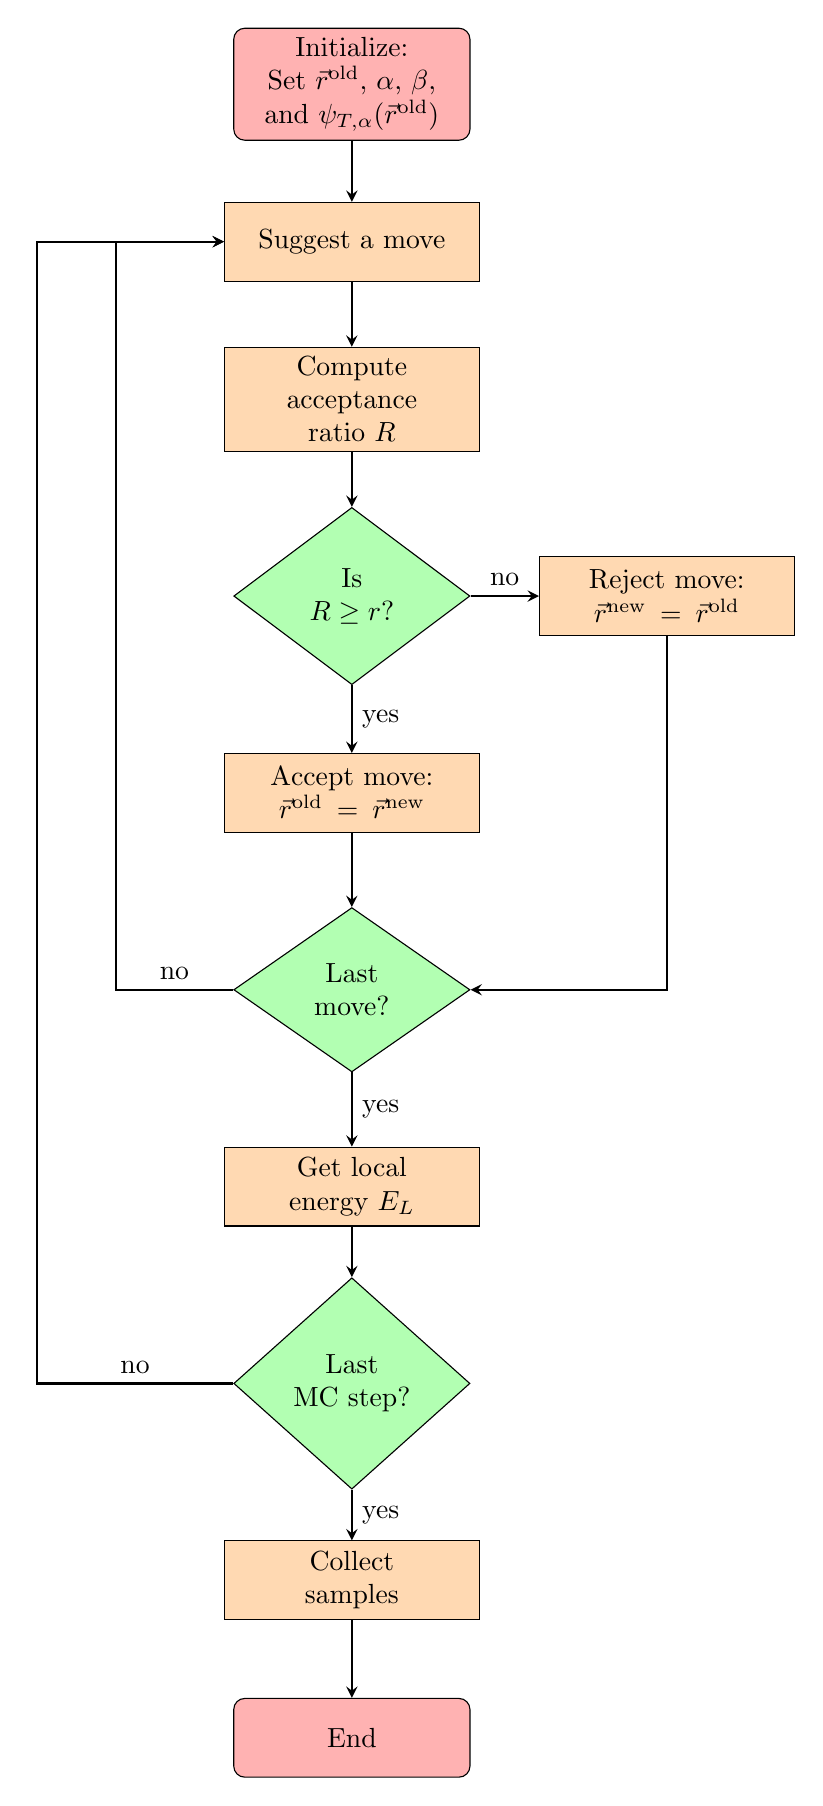
\begin{tikzpicture}[node distance=2cm]
	
		% Draw the nodes
		\node (start) [startstop, align=center] {Initialize:\\ Set $\vec{r}^{\text{old}}$, $\alpha$, $\beta$,\\ and $\psi_{T,\alpha}(\vec{r}^{\text{old}})$};
		%\node (in1) [io, below of=start] {Input};
		\node (pro1) [process, below of=start] {Suggest a move};
		\node (pro2) [process, below of=pro1] {Compute\\ acceptance\\ ratio $R$};
		\node (dec1) [decision, below of=pro2, yshift=-0.5cm, align=center] {Is\\$R \geq r$?};
		\node (pro3a) [process, below of=dec1, yshift=-0.5cm, align=center] {Accept move:\\ $\vec{r}^{\text{old}} = \vec{r}^{\text{new}}$};
		\node (pro3b) [process, right of=dec1, xshift=2cm] {Reject move:\\ $\vec{r}^{\text{new}} = \vec{r}^{\text{old}}$};
		\node (dec2) [decision, below of=pro3a, yshift=-0.5cm, align=center] {Last\\ move?};
		\node (dec2left) [left of=dec2, xshift=-1cm] {};
		\node (pro5) [process, below of=dec2, yshift=-0.5cm] {Get local\\ energy $E_L$};
		\node (dec3) [decision, below of=pro5, yshift=-0.5cm, align=center] {Last\\ MC step?};
		\node (dec3left) [left of=dec3, xshift=-2cm] {};
		\node (pro6) [process, below of=dec3, yshift=-0.5cm, align=center] {Collect\\ samples};
%		\node (out1) [io, below of=pro2a] {Output};
		\node (stop) [startstop, below of=pro6] {End};
		
		%Draw the arrows
		\draw [arrow] (start) -- (pro1);
		\draw [arrow] (pro1) -- (pro2);
		\draw [arrow] (pro2) -- (dec1);
		\draw [arrow] (dec1) -- node[anchor=west] {yes} (pro3a);
		\draw [arrow] (dec1) -- node[anchor=south] {no} (pro3b);
		\draw [arrow] (pro3b) |- (dec2);
		\draw [arrow] (pro3a) -- (dec2);
		\draw [arrow] (dec2) -- node[anchor=west] {yes} (pro5);
		\draw [arrow] (dec2) -- node[anchor=south] {no} (dec2left.center) |- (pro1);
		\draw [arrow] (pro5) -- (dec3);
		\draw [arrow] (dec3) -- node[anchor=west] {yes} (pro6);
		\draw [arrow] (dec3) -- node[anchor=south] {no} (dec3left.center) |- (pro1);
		\draw [arrow] (pro6) -- (stop);
	
	\end{tikzpicture}
	\caption{Quantum Variational Monte Carlo algorithm.}
	\label{fig:chart_flow}
\end{figure}

\clearpage

\begin{figure}[p]
    \centering
    \includegraphics[width=1.0\textwidth]{performance2OLD.png}
    \caption{Old performance N=2}
\end{figure}

\clearpage

\begin{figure}[p]
    \centering
    \includegraphics[width=1.0\textwidth]{performance2.png}
    \caption{Current performance N=2, 3.8x speed up.}
\end{figure}

\clearpage


\begin{figure}[p]
    \centering
    \includegraphics[width=1.0\textwidth]{performance6OLD.png}
    \caption{Old performance N=6}
\end{figure}

\clearpage

\begin{figure}[p]
    \centering
    \includegraphics[width=1.0\textwidth]{performance6.png}
    \caption{Current performance N=6, 22.3x speed up.}
\end{figure}

\clearpage






\end{document}
